\subsection{Book Extraction}
To extract the set of points that represented the book we used couple of thresholds in order to capture the book and reduce noise. First, we used the point cloud that can be seen in Figure \ref{fig:points} and subtracted the points belonging to the three planes. The, to eliminate other data points, such as outside the cabinet (see Figure \ref{fig:regionGrowing}), we subtracted all points that were to the left and right of the topmost plane, and ones that were below the corner point. Finally, to eliminate noise on the topmost plane, we extracted only the points that had the distance $\geq 1$ from the top plane. The result for our foundation frame, where the book extraction worked well, can be seen in Figure \ref{fig:bookPoints}.

\begin{figure}[H]
	\centering
	\begin{subfigure}[b]{0.45\textwidth}
		\centering
		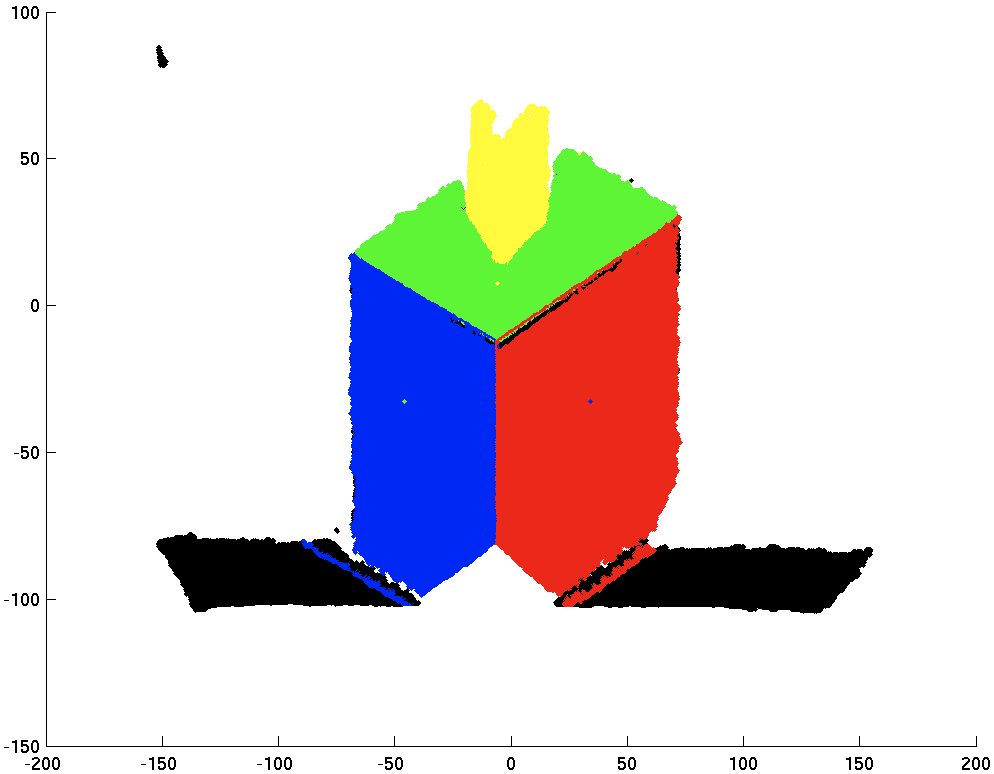
\includegraphics[width=\textwidth]{Images/6-BookPoints(1).png}
		\subcaption{}
		\label{fig:bookPoints}
	\end{subfigure}%
	\hspace{1cm}
	\begin{subfigure}[b]{0.45\textwidth}
		\centering
		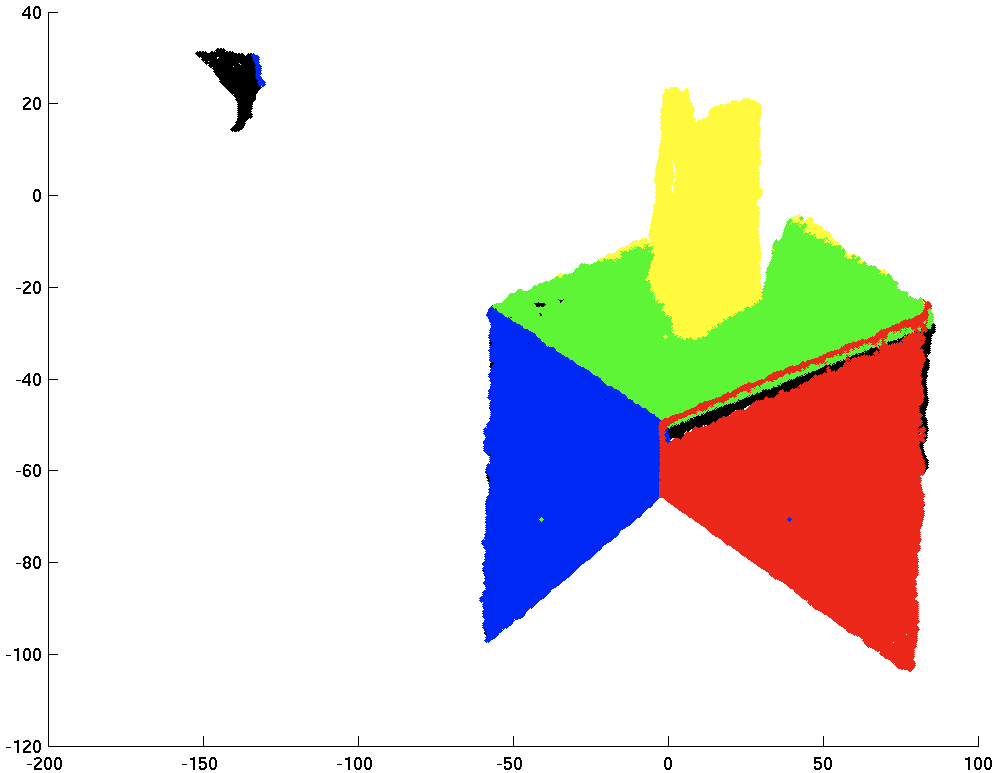
\includegraphics[width=\textwidth]{Images/6-BookPoints-frame2(1).png}
		\subcaption{}
		\label{fig:bookPointsFrame2}
	\end{subfigure}
	\caption{Book points for the foundation frame 17 (a) and frame 2 (b) displayed in yellow.}
\end{figure}

An example of a frame for which the book extraction worked less well (frame 2) is shown in figure \ref{fig:bookPointsFrame2}. In this figure it is apparent that there are a number of yellow points on the top plane that are not actually part of the book.

To fix this, we created a recursive algorithm that used a region growing approach to distinguish true book points from noise, based on the following two observations:

\begin{itemize}
	\item The true book points form a coherent group, in which each point is close to some other point in the book, while the noise points are relatively spread out
	\item The highest point in the image is always a true book point, as the noise points are seen close to the cabinet
\end{itemize}

The algorithm defined a frontier set of points, initialized as a singleton set comprising the highest point. On each iteration the algorithm generated a new frontier set, comprising points that were within a set euclidean distance (12 in our case) from some member of the previous frontier set. The algorithm terminates when the new frontier set is empty. The resulting set of true book points is the union of all of the frontier sets, and is built incrementally as the algorithm runs. The result of running this algorithm on the noisy set of book points in frame 2 is shown in figure \ref{fig:bookPointsFrame2Cleaned}, with the true book points shown in red, and the noise points in black.


\begin{figure}[H]
	\centering
	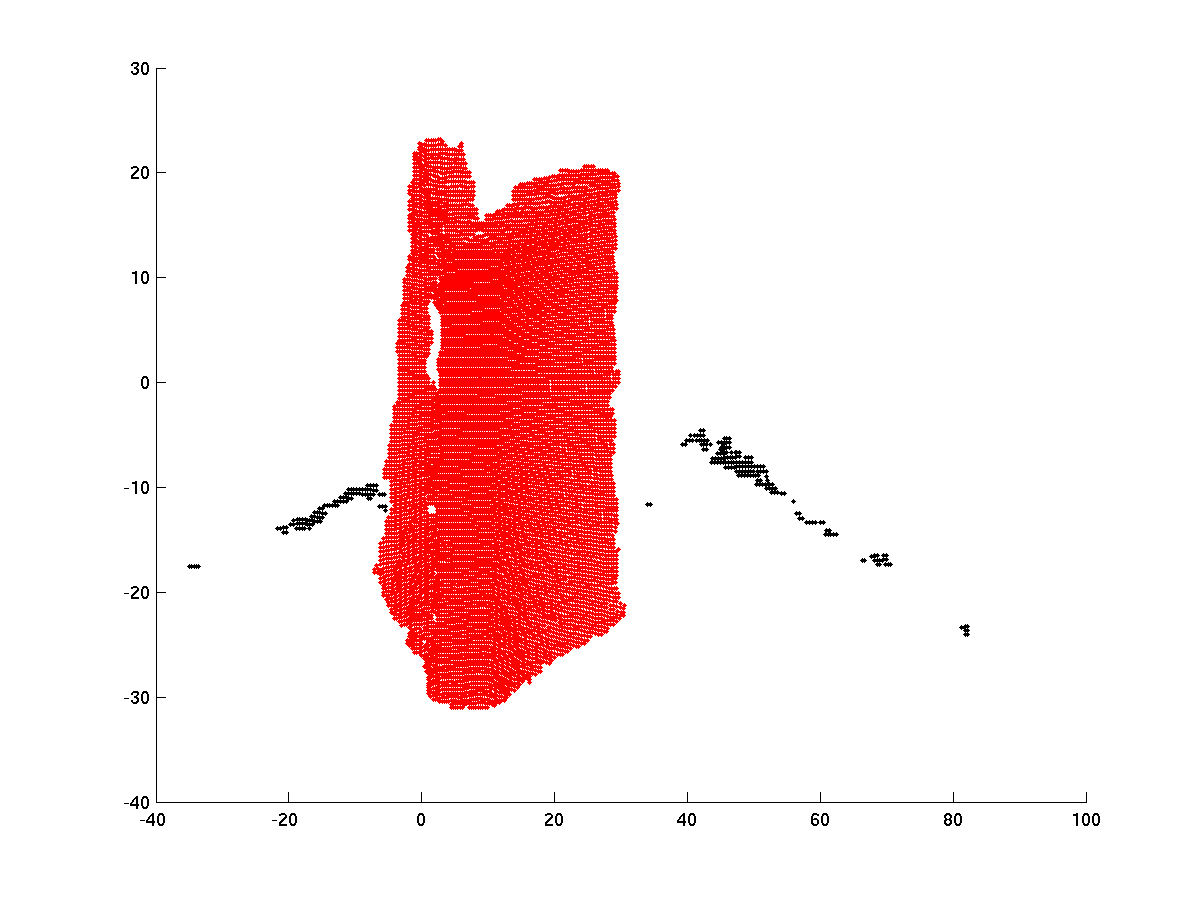
\includegraphics[width=0.5\textwidth]{Images/6-RegionGrowingCleaning.png}
	\caption{Extracted book points for frame 2 after an additional recursive algorithm for region growing has been applied to distinguish true book points from noise. True book points are shown in red.}
	\label{fig:bookPointsFrame2Cleaned}
\end{figure}

The matlab code to perform the book extraction is shown in section \ref{BookExtractionCode} of this report.